\documentclass[12pt,a4paper]{report}

\usepackage[spanish]{babel}
\usepackage[utf8]{inputenc}
\usepackage{dad}

\title{Desarrollo de Aplicaciones Distribuidas: \\ Registrador de juegos}
\author{Rafael Gálvez-Cañero, Andreas Gerstmayr}
\date{Iteración 4 - 7 de Abril de 2015} % delete this line to display the current date



%%% BEGIN DOCUMENT
\begin{document}
\maketitle
\tableofcontents
\listoffigures
\listoftables

\pagenumbering{arabic}

% Esto representa la primera iteración (capítulo), información general
\chapter{Datos generales}

\section{Miembros del grupo}

\begin{table}[htdp]
\begin{center}
\begin{tabular}{|l|l|l|c|}
\hline
\textbf{Apellidos}&\textbf{Nombre}&\textbf{Correo-e}&\textbf{Grupo}\\
\hline
Gálvez-Cañero&Rafael&\href{mailto:galvesband@gmail.com}{galvesband@gmail.com}&18\\
Gerstmayr&Andreas&\href{mailto:andreas.gerstmayr@gmail.com}{andreas.gerstmayr@gmail.com}&18\\
\hline
\end{tabular}
\end{center}
\caption{Miembros del grupo}
\label{tab:miembros}
\end{table}%


\section{Descripción del sistema}

\begin{itemize}
\item \textbf{Tipo de sistema distribuido}:
\item \textbf{Nombre del proyecto}: Plataforma de juegos, Game Register
\item \textbf{Breve descripción}: Sub-sistema para registrar sesiones de juego e información asociada.
\end{itemize}

\subsection{Funcionalidad observable}

\begin{itemize}
\item Registrar el inicio y el término de todas las sesiones de juego.
\item Visualizar el historial de juegos.
\item Visualizar qué jugadores juegan en este momento.
\end{itemize}

\subsection{Servicios ofrecidos}
\begin{itemize}
\item Servicio de Registro: Capacidad de aceptar la información de una sesión de juego.
\item Servicio de Historial: Ofrece métodos para consultar el historial de sesiones.
\item Servicio de Sesiones Online: Muestra una lista de jugadores actualmente en activo.
\end{itemize}

\subsection{Servicios demandados}
\begin{itemize}
\item Servicio X: breve descripción. Fecha aproximada a partir de la que se necesitará (si se conoce).
\item Servicio Y: idem.
\end{itemize}

\section{Direcciones de descarga y planificación}

\begin{table}[htdp]
\begin{center}
\begin{tabular}{|c|c|}
\hline
\textbf{Código fuente}&\url{https://repositorio.informatica.us.es/svn/lq3vqrtzfnh2nx9yhpk}\\
\hline
\multicolumn{2}{|c|}{\textbf{Planificación temporal}}\\
\hline
Iteración 1&17/02/2015\\
Iteración 2&01/03/2015\\
Iteración 3&15/03/2015\\
Iteración 4&05/04/2015\\
Iteración 5&19/04/2015\\
Iteración 6&10/05/2015\\
Iteración 7&24/05/2015\\
Entrega Final&07/06/2015\\
\hline
\end{tabular}
\end{center}
\caption{Datos generales del trabajo en grupo}
\label{tab:datosgenerales}
\end{table}%

\section{Seguimiento}

\begin{table}[htdp]
\begin{center}
\begin{tabular}{|c|c|c|c|c|c|c|c|c|c|c|c|}
\cline{2-10}
\multicolumn{1}{c}{}&\multicolumn{9}{|c|}{\textbf{Iteración}}&\multicolumn{2}{c}{}\\
\hline
\textbf{Estudiante}&1&2&3&4&5&6&7&8&Final&Total&Pond.\\
\hline
Rafael Gálvez-Cañero&5&5&5&5&5&5&5&5&5&\textbf{40}&1\\
Andreas Gerstmayr&5&5&5&5&5&5&5&5&5&\textbf{40}&1\\
\hline
Total&30&30&30&30&30&30&30&30&\multicolumn{2}{c}{}\\
\cline{1-9}
\end{tabular}
\end{center}
\caption{Tabla de seguimiento}
\label{tab:seguimiento}
\end{table}%


% Segunda iteración (capítulo), diagramas UML de clases y despliegue
\chapter{Modelado}

\section{Análisis del sistema}
 \begin{center}
  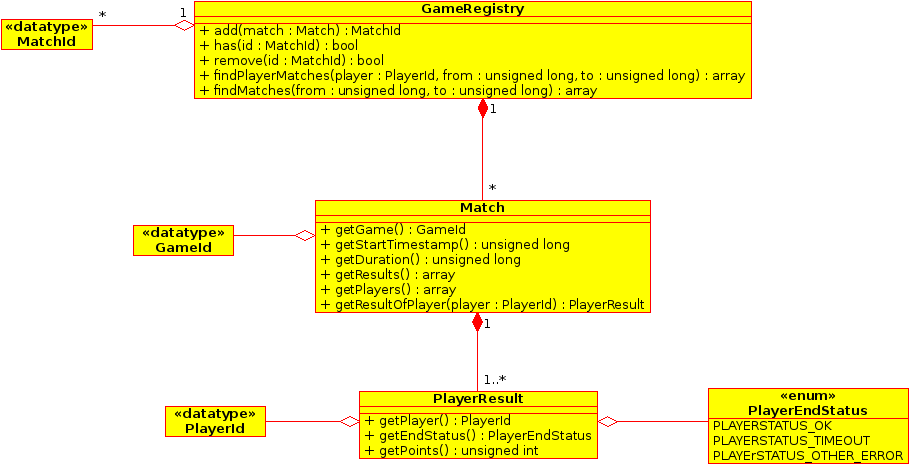
\includegraphics[scale=0.6]{./class_diagram.png}
  % class_diagram.png: 0x0 pixel, 300dpi, 0.00x0.00 cm, bb=
 \end{center}


\section{Arquitectura del sistema}
\begin{figure}[h]
 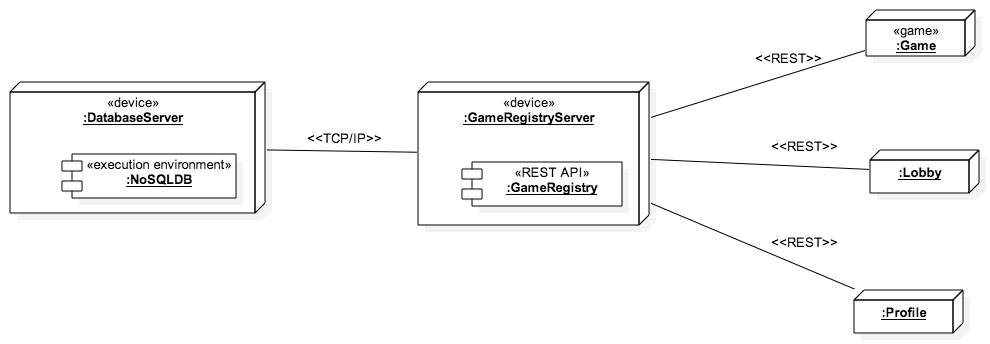
\includegraphics[scale=0.5]{diagrams/deployment_diagram.png}
 \caption{Modelo de despliegue del sistema}
 \label{fig:arquitectura}
\end{figure}


% Tercera iteración (gradle, dockerización)
\chapter{Iteración 3}
\section{Objetivos de iteración}
\begin{itemize}
  \item Integración de Gradle 
  \item Servidor dockerizado
  \item Estructura inicial del Cliente vertx.
\end{itemize}

\section{Gradle}
\emph{Gradle} es un gestor de construcción especialmente indicado para proyectos
Java y con soporte para \emph{Groovy}, \emph{Vertx} y \emph{Maven}.

Ha sido integrado mediante el wrapper \texttt{gradlew} que permite utilizar Gradle sin
instalarlo de forma global en el sistema de desarrollo. La primera vez que se
lanza descargará todas las bibliotecas necesarias.

En el archivo \textbf{Readme.md} hay información básica sobre como construir el
proyecto. Algunos comandos útiles:

\begin{itemize}
 \item Para \textbf{construir} el proyecto: \\
       \texttt{\$ ./gradlew clean modZip}
 \item Para \textbf{lanzar} el servidor en la máquina local: \\
       \texttt{\$ ./gradlew runMod -i}
 \item Para lanzar los \textbf{tests}: \\
       \texttt{\$ ./gradlew clean test}
 \item Para preparar el proyecto para un \textbf{entorno de desarrollo}:
    \begin{itemize}
      \item Eclipse: \texttt{\$ ./gradlew eclipse}
      \item IDEA: \texttt{\$ ./gradlew idea}
    \end{itemize}
\end{itemize}

\section{Dockerización}
\emph{Docker} es una tecnología que permite utilizar contenedores sobre \emph{Linux} para
ejecutar procesos de forma aislada y con un runtime reproducible.

Nuestro proyecto proporciona un archivo \textbf{Dockerfile} con las instrucciones necesarias
para construir el contenedor de la aplicación. Además, el archivo \textbf{Readme.md} contiene
información sobre el procedimiento para lanzar el proyecto en \emph{Docker}. 

El procedimiento para lanzar el servidor con \emph{Docker} ahora mismo es el siguiente:

\begin{itemize}
 \item Limpiar y contruir el proyecto: \\
       \texttt{\$ ./gradlew clean modZip}
 \item Construir el contenedor con el servidor: \\
       \texttt{\$ docker build -t distributedsystems/gameregistry .} \\
       (notar el punto final del comando que indica a \emph{Docker} dónde buscar el archivo
       \emph{Dockerfile} con las instrucciones de construcción). La construcción incluye el 
       resultado de compilación del proyecto por lo que cada vez que este cambie el contenedor
       debe ser reconstruido.
 \item Lanzar el contenedor del servidor: \\
       \texttt{\$ docker run distributedsystems/gameregistry}
\end{itemize}


% Cuarta iteración (mongo, reestructuración de servidor en Servicio / Controlador / Dominio)
%!TEX root =  MemoriaGrupo00.tex
% --------------------------------------------
% Iteraci�n 4
% --------------------------------------------
\chapter{Iteraci�n 4}

\section{Planificaci�n}
\section{Dise�o}
\subsection{Diagrama de clases UML}

\begin{figure}[htbp]
\begin{center}
\missingfigure{Aqu� el modelo de dise�o en formato vectorial preferentemente (pdf)}
% Incluir la figura quitando el comentario a la fila de abajo.
% \includegraphics[width=\textwidth]{myfile.pdf}
\caption{Diagrama UML de dise�o para la iteraci�n 4}
\label{fig:diseno03}
\end{center}
\end{figure}

\subsection{Documentos de asignaci�n de responsabilidades}

\subsection{Memorandos t�cnicos}

\section{Informaci�n adicional}


\chapter{Iteracion 5}
\section{Objetivos de iteración}
\begin{itemize}
  \item Implementación inicial de API
  \item Primeros tests.
  \item Despliegue Azure plataforma
  \item ¿Integración contínua?
\end{itemize}

\section{Diagrama de despliegue}
\begin{center}
 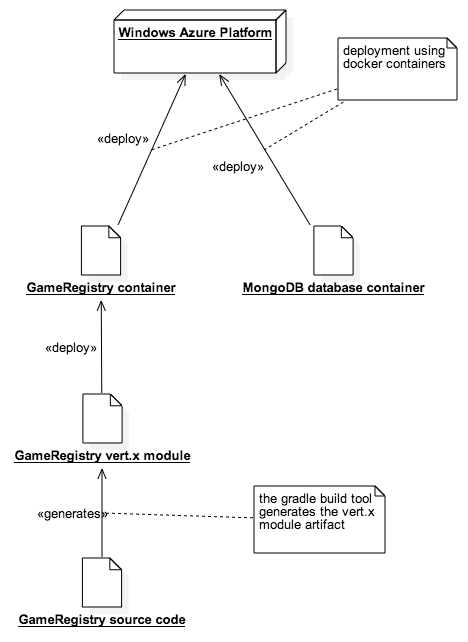
\includegraphics[scale=0.6]{diagrams/docker_deployment_diagram.png}
\end{center}
 
\chapter{Iteracion 6}
\section{Objetivos de iteración}
Final testing.

\chapter{Iteracion 7}
\section{Objetivos de iteración}
Subir a repositorio Maven.

\end{document}
\appendix

\chapter{Documentación de API MyService}

Aquí el texto que se considere necesario.
